% Standalone TikZ source for AMP architecture diagram.
% Build: tectonic -X compile architecture.tex  (or pdflatex)
\documentclass[tikz,border=10pt]{standalone}
\usepackage{tikz}
\usetikzlibrary{positioning,arrows.meta,shapes,fit,backgrounds,calc}

\begin{document}
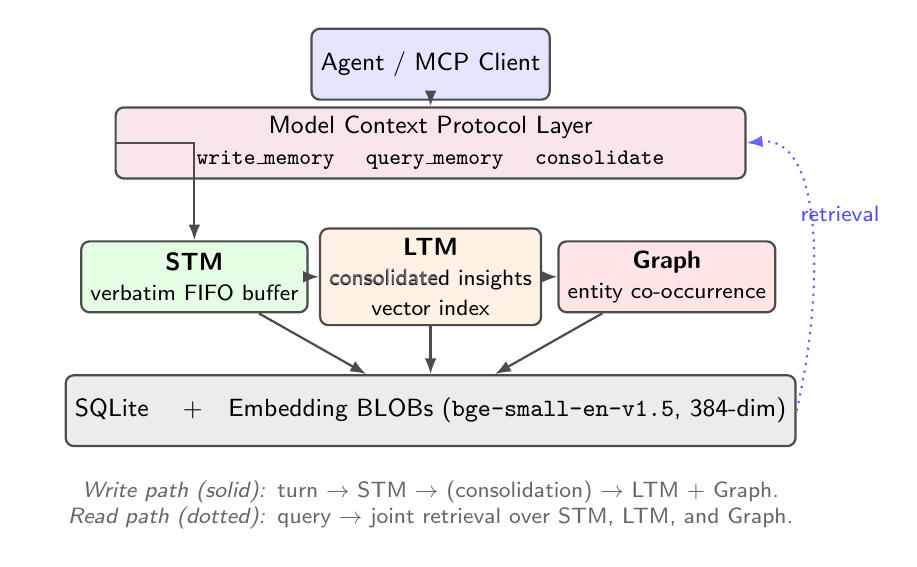
\begin{tikzpicture}[
    font=\small\sffamily,
    box/.style={rectangle, rounded corners=3pt, draw=black!70, thick, minimum width=2.6cm, minimum height=0.9cm, align=center, fill=white},
    layer/.style={rectangle, rounded corners=5pt, draw=black!50, thick, fill=#1, inner sep=10pt},
    arr/.style={-{Latex[length=2mm]}, thick, draw=black!70},
    label/.style={font=\footnotesize\sffamily, text=black!60}
]

% Top: Agent / Client
\node[box, fill=blue!10] (agent) at (0, 5.4) {Agent / MCP Client};

% MCP Protocol bar
\node[box, minimum width=8cm, fill=purple!10] (mcp) at (0, 4.4) {Model Context Protocol Layer \\ \footnotesize\texttt{write\_memory} \quad \texttt{query\_memory} \quad \texttt{consolidate}};

% Three layers
\node[box, fill=green!10, minimum width=2.4cm] (stm) at (-3, 2.7) {\textbf{STM} \\ \footnotesize verbatim FIFO buffer};
\node[box, fill=orange!10, minimum width=2.4cm] (ltm) at (0, 2.7) {\textbf{LTM} \\ \footnotesize consolidated insights \\ \footnotesize vector index};
\node[box, fill=red!10, minimum width=2.4cm] (graph) at (3, 2.7) {\textbf{Graph} \\ \footnotesize entity co-occurrence};

% Storage backend
\node[box, minimum width=8cm, fill=gray!15] (storage) at (0, 1.0) {SQLite \quad+\quad Embedding BLOBs (\texttt{bge-small-en-v1.5}, 384-dim)};

% Arrows: write path
\draw[arr] (agent) -- (mcp);
\draw[arr] (mcp) -| (stm);
\draw[arr, dashed] (stm) -- node[label, right=2pt]{consolidate} (ltm);
\draw[arr, dashed] (ltm) -- (graph);
\draw[arr] (stm) -- (storage);
\draw[arr] (ltm) -- (storage);
\draw[arr] (graph) -- (storage);

% Read path back
\draw[arr, dotted, thick, draw=blue!60] (storage.east) .. controls (5, 2.5) and (5, 4.5) .. (mcp.east);

% Annotation: read path
\node[label, text=blue!70] at (5.2, 3.5) {retrieval};

% Caption box (optional)
\node[label, text width=10cm, align=center] at (0, -0.2) {%
\textit{Write path (solid):} turn $\to$ STM $\to$ (consolidation) $\to$ LTM + Graph. \quad \textit{Read path (dotted):} query $\to$ joint retrieval over STM, LTM, and Graph.};

\end{tikzpicture}
\end{document}
